\documentclass[conference]{IEEEtran}
\usepackage{cite}
\usepackage{amsmath,amssymb,amsfonts}
\usepackage{algorithmic}
\usepackage{graphicx}
\usepackage{textcomp}
\usepackage{xcolor}
\def\BibTeX{{\rm B\kern-.05em{\sc i\kern-.025em b}\kern-.08em
    T\kern-.1667em\lower.7ex\hbox{E}\kern-.125emX}}
\begin{document}
\selectlanguage{dutch}

\title{Digitale kunstcollecties ontdekken door middel van Link-Traversal–based Query Processing}

\author{\IEEEauthorblockN{Martijn Bogaert}
\IEEEauthorblockA{
\textit{Universiteit Gent}\\
Gent, België \\
martijn.bogaert@ugent.be}}

\maketitle

\begin{abstract}
TODO
\end{abstract}

\begin{IEEEkeywords}
TODO
\end{IEEEkeywords}

\section*{Inleiding}
TODO

\section{Gerelateerd werk}
TODO

\subsection{Collectie van de Gentenaar}
TODO

\subsection{International Image Interoperability Framework}
TODO

\subsection{Link-Traversal-based Query Processing}
TODO

\section{CoGent data en link traversal}
TODO

\subsection{CoGent databronnen}
TODO

\subsection{Comunica link traversal engine configuratie}
TODO

\subsection{Te volgen links}
TODO

\section{Tools voor de constructie van query's}
TODO

\subsection{Queryconstructie door middel van predicaatsequenties}
TODO

\subsection{Gebruikersgerichte applicaties}
TODO

\section{Queryresultaten verwerken}
TODO

\subsection{Queryresultaten visualiseren}
TODO

\subsection{Queryresultaten opslaan}
TODO

\section*{Dankwoord}
TODO

% \bibliographystyle{IEEEtran}
% \bibliography{references}

\end{document}


% \begin{table}[htbp]
% \caption{Table Type Styles}
% \begin{center}
% \begin{tabular}{|c|c|c|c|}
% \hline
% \textbf{Table}&\multicolumn{3}{|c|}{\textbf{Table Column Head}} \\
% \cline{2-4} 
% \textbf{Head} & \textbf{\textit{Table column subhead}}& \textbf{\textit{Subhead}}& \textbf{\textit{Subhead}} \\
% \hline
% copy& More table copy$^{\mathrm{a}}$& &  \\
% \hline
% \multicolumn{4}{l}{$^{\mathrm{a}}$Sample of a Table footnote.}
% \end{tabular}
% \label{tab1}
% \end{center}
% \end{table}

% \begin{figure}[htbp]
% \centerline{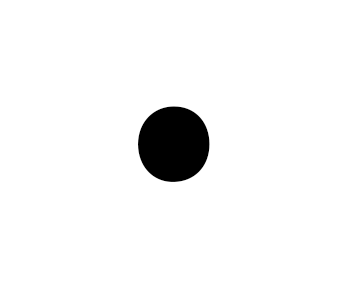
\includegraphics{fig1.png}}
% \caption{Example of a figure caption.}
% \label{fig}
% \end{figure}